\chapter{}\label{ch:ch1}
\section{Состояние исследований в области динамических воздействий на оптико-электронные системы КА}

В последние годы в научной инженерной среде возрастает интерес к повышению точности и разрешающей способности космических средств наблюдения, предназначенных для дистанционного зондирования Земли (ДЗЗ) и определения малоэнергетических целей \cite{haroon2020multisized, bouwmeester2023enabling, saunders2017building, cheng2024geometric, hamm2015earth}. Одним из основных направлений является увеличение размеров оптических систем и внедрения механизмов изменения положения визирной оси без поворота КА \cite{kandepi2024agile, franze2023attitude}.

Поворот визирной оси может выполняться различными способами:
\begin{itemize}
	\item разворотом всего КА;
	\item перемещением отдельных элементов оптической системы;
	\item использованием карданных механизмов \cite{leskov2010kardan,negro2023inertial}
\end{itemize}

Независимо от выбранной схемы, перемещение подвижных масс вызывает возникновение реактивных сил и моментов, передающихся на корпус аппарата, вызывая угловые отклонения и колебания. Это затрудняет работу системы стабилизации, а также снижают пространственное разрешение и контрастность изображения за счет \blur{} и вибрационных искажений  \cite{lappas2002attitude, углова2019оценка, zhao2023effect} Особенно критично это для инфракрасных и широкоформатных систем, имеющих большие габариты и массу \cite{shorthill1990infrared. shivanandan1985far}.   \cite{pittelkau2012pointing, dennehy2021spacecraft, alvarez2018spacecraft}.

Качество изображения, формируемого оптико-электронным каналом, характеризуется совокупностью радиометрических и геометрических параметров, среди которых ключевыми считаются функция передачи модуляции (ФПМ), отношение сигнал/шум и интегральный показатель Image Quality Factor (IQF) \cite{leachtenauer1997general}. Последний определяется как произведение отношения сигнал/шум на суммарную ФМП сквозного информационного тракта \cite{}:
\begin{equation}
	\label{eq:eq_IQF}
	 IQF(v)=SNR(v)\cdot MFP(v)
\end{equation}
	где \( v \) "--- пространственная частота, \( MFP \) "--- суммарная функция передачи модуляции, \( SNR \) "---отношение сигнал/шум.

Снижение ФПМ при относительном движении изображения описывается зависимостью \cite{}
	
\begin{equation}
	\label{eq:eq_MTF}
	MTF(v)=\frac{\sin (\pi \alpha v')}{\pi \alpha v'}
\end{equation}
где \(\alpha\) "--- смещение изображения за время экспозиции, \(v'\) "--- проекция вектора частоты с учётом ориентации вектора смещения. При высокочастотных колебаниях используется функция Бесселя нулевого порядка \cite{}:

\begin{equation}
	\label{eq:eq_Bessel}
	T(v)=J_0(2\pi \alpha v)
\end{equation}

где \(\alpha\) "--- амплитуда колебаний.

Источники вибраций и смаза связаны с работой приводов визирной оси, дисбалансами маховиков, погрешностями редукторов и взаимодействием с гибкими элементами конструкции КА \cite{}

В мировой практике для компенсации реактивных моментов применяются реактивные маховики и гиродины \cite{}, балансировка подвижных узлов \cite{}, а также алгоритмы управления приводами \cite{}. Эти методы позволяют снизить спектр возмущений в критических диапазонах частот, но не исключают полностью влияния на качество изображения % todo Переписать

 

\section{Влияние реактивного момента на \blur{} изображения}

Одним из наиболее значимых факторов, ухудшающих качество изображений в оптико-электронных системах космического назначения, является \blur{} — размывание деталей изображения, вызванное несоответствием скорости движения изображения по фокальной плоскости приёмника тактовому периоду опроса.

В оптико-электронных сканирующих системах (ОЭСС) с приборами с зарядовой связью (ПЗС) смаз возникает, когда за время экспозиции фоточувствительный элемент принимает излучение не только от «своей» проекции участка поверхности, но и от смежных. Это приводит к интегрированию сигналов от разных элементов сцены и, как следствие, к снижению резкости, контрастности и читаемости мелких деталей.

Для исключения \blur{} необходимо, чтобы за один тактовый период опроса $\tau_T$ смещение изображения $\Delta$, обусловленное орбитальным перемещением космического аппарата, было равно размеру проекции соседних элементов ПЗС-матрицы на Землю:

\begin{equation}
	\label{eq:eq_blurPSZ}
	\Delta(\tau_T) = L = l_x \cdot m_c,
\end{equation}

где \(l_x\) "--- линейный размер пикселя по направлению сканирования, \(m_c\) "--- масштаб изображения. 

Оптимальный тактовый период опроса определяется по расчётной скорости движения изображения $v_0$:
\begin{equation}
	\label{eq:eq_optimalPeriod}
	\tau_T^* = \frac{L}{v_0} = \frac{l_x m_c}{v_0}.
\end{equation}

При $\tau_T > \tauopt{T}$ смещение меньше $L$, и сигнал одного участка сцены накапливают несколько пикселей, что вызывает продольное размытие. При $\tau_T < \tauopt{T}$ смещение превышает $L$, и часть информации теряется между пикселями, что приводит к потере мелких деталей. в "разреживании" % todo исправить 
структуры изображения (снижается резкость и контрастность мелких деталей).

% todo РИСУНКИ пикселбной структуры

В режиме временной задержки и накопления (ВЗН) перенос зарядовых пакетов выполняется синхронным опросом всех строк ПЗС-матрицы, причем между тактами элементы продолжают экспонироваться закреплёнными за ними участками сцены. В момент опроса одновременно происходят два процесса -- перенос ранее сформированных зарядов в следующую строку и считывание сигналов с первой строки в бортовой вычислительный комплекс. Такая организация работы чувствительных элементов обуславливает высокую чувствительность режима ВЗН к рассогласованию между скоростью движения изображения и частотой опроса.

Величина \blur{} в пространственных единицах может быть выражена через линейное смещение изображения $\alpha=v\tau_T$ в плоскости матрицы. Функция передачи модуляции при направленном \blur{} задаётся зависимостью:

\begin{equation}
	\label{eq:eq_FPMblur}
	T(v,\alpha)=\frac{\pi \alpha v'}{\pi \alpha v'}, \quad v'=v \cdot \cos \varphi
\end{equation}

где \(v\) "--- скорость движения изображения, \(\varphi\) "--- угол между направлением движения изображения и строками приёмника. 

Даже небольшое смещение $\alpha$, сравнимое с размером пикселя, приводит к заметному снижению пространственной частотной характеристики %todo дописать понятное объяснение

Рассогласование между фактическим и расчётным тактовым периодом $\tau_T$ может быть вызвано методическими ошибками расчёта СДИ, неточностью поддержания орбитальной и угловой ориентации, температурными деформациями конструкции и вибрациями. В контексте настоящего исследования особое внимание уделено возмущениям, возникающим при поворотах подвижных частей оптической системы.

Поворот оптической системы осуществляется моментом, формируемым приводом, который через реакцию механических связей оказывает  такой же по значению и противоположный по знаку момент на корпус космического аппарата. Этот момент изменяет  угловую скорость КА из-за чего изменяется скорость движения изображения на фокальной плоскости. Изменение скорости определяется как:

\begin{equation}
	\label{eq:eq_spdiimage}
	v = f \cdot \omega_{||}
\end{equation}

где \(f\) "--- фокусное расстояние оптической системы, \(\omega_{||}\) "--- проекция угловой скорости на направление сканирования.

Воздействие реактивного момента можно разделить на 3 составляющие:

\begin{enumerate}
	\item Постоянная составляющая -- низкочастотное изменение угловой скорости, которое изменяет среднее значение СДИ  и вызывает систематический \blur по всей полосе съёмки. 
	\item Гармоническая составляющая -- колебания, вызванные резонансами конструкции. Влияние на ФПМ описывается выражением:
	\begin{equation}
		\label{eq:eq_fmpHarmonic}
		T_{\text{harm}} = J_0(2\pi a_{\sin} v),
	\end{equation}
	где \(a_{\sin}\) "--- амплитуда смещения изображения от колебаний, \(J_0\) "--- функция Бесселя нулевого порядка.
	\item Случайная составляющая -- возмущения вызванные нерегулярной работы приводов и механическими шумами. Влияние на ФПМ описывается так:
	\begin{equation}
		\label{eq:eq_fmpExp}
		T_{\text{rand}} = \exp(-2\pi^2 \sigma_R^2 v^2),
	\end{equation}
	
	где \(\sigma_R\) "--- среднеквадратическое значение дрожания изображения. 
\end{enumerate}

Все перечисленные компоненты реактивного момента вносят вклад в снижение функции передачи модуляции и интегральных показателей качества, таких как Image Quality Factor, и требуют разработки специальных мер компенсации. Таким образом, \blur{} в оптико-электронных системах является наглядным проявлением воздействия реактивного момента на процесс формирования изображения.



Нарушение условия $\tauopt{T} = \tau_T$ приводит к двум сценариям \blur{а}:
\begin{itemize}
	\item при $\tau_T > \tauopt{T}$ смещение изображения меньше $L$, сигнал одного участка сцены накапливают несколько пикселей, что даёт продольное размытие;
	\item при $\tau_T < \tauopt{T}$ смещение больше $L$, часть информации теряется между пикселям, что выражается в "разреживании" % todo исправить 
	структуры изображения (снижается резкость и контрастность мелких деталей).
\end{itemize}

% todo РИСУНКИ пикселбной структуры

Важная особенность режима ВЗН -- перенос зарядовых пакетов выполняется синхронным опросом всех строк ПЗС-матрицы, причем между тактами элементы продолжают экспонироваться своими участками сцены. В момент опроса параллельно происходит два процесса -- перенос ранее сформированных ЗП в следующую строку и считывание зарядовых пакетов с первых строк в бортовой вычислительный комплекс. Такая организация работы чувствительных элементов обуславливает особую чувствительность режима ВЗН к рассогласованию между скоростью движения изображения и частотой опроса.

Величина \blur{а} может быть выражена через линейное смещение изображения $\alpha=v\tau_T$ в плоскости матрицы. Функция передачи модуляции при направленном \blur{е} задается зависимостью \cite{}:

\begin{equation}
	\label{eq:eq_FPMblur}
	T(v,\alpha)=\frac{\sin(\pi \alpha v')}{\pi \alpha v'}
\end{equation}

где \(v\) "--- скорость движения, \(v'=v\cdot \cos \alpha\), \(\alpha\) "--- угол между направлением движения изображения и строками приёмника. 
Эта функция показывает, что даже небольшое смещение $\alpha$, сравнимое с размером пикселя, приводит к заметному снижению пространственной частотной характеристики системы.

Практика эксплуатации оптикао-электронных сканирующих систем показывает, что рассогласование между фактическим и расчётным тактовым периодом может быть вызвано целым комплексом факторов --
методическими ошибками расчёта скорости движения изображения,неточностью поддержания орбитальной и угловой ориентации, температурными деформациями конструкции,вибрациями. Особо сильное влияние оказывают  возмущения, возникающие в вращения подвижных частей самой оптической системы (поворот визирной оси на заданный угол). Вращение оптической системы, вызывает реактивный момент, воздействующий на корпус КА. Под действием этого момента, ориентация КА %todo дописать.
Это приводит к изменению продольной и поперечной составляющей скорости движения изображения. В результате фактическое значение тактового периода $\tau_T$ перестаёт соответствовать оптимальному $\tauopt{T}$ и в процессе сканирования начинает накапливаться \blur{}.
Реактивный момент при вращении вносит в движение изображения как постоянную составляющую смещения, так и переменные компоненты, имеющие гармонический или случайный характер. Влияние гармонических составляющих на ФПМ описывается так:

\begin{equation}
	\label{eq:eq_fmpHarmonic}
	T_{harm}=J_0(2\pi\alpha_{\sin}v)	
\end{equation}
где \(\alpha_{\sin}\) "--- амплитуда смещения изображения от колебаний, \(J_0\) "--- функция Бесселя нулевого порядка.

Случайные возмущения, например,вызванные неравномерностью работы приводов, приводят к экспоненциальному снижении модуляции:

\begin{equation}
	\label{eq:eq_fmpExp}
	T_{rand}=exp(-2\pi^2\sigma_R^2v^2)
\end{equation}

где \(\sigma_R\) "--- среднеквадратичное значение дрожания изображения.

Оба этих эффекта приводят к падению интегральных показателей качества изображения, таких как Image Quality Factor, и требуют специальных мер компенсации.

Таким образом, \blur в оптико-электронных системах является наглядным проявлением воздействия реактивного момента на процесс формирования изображения.

Реактивный момент в космических аппаратах возникает как следствие действия закона сохранения момента количества движения. При вращении оптической системы создается управляющий момент с помощью приводов. Этот момент вызывает реакцию со стороны корпуса аппарата или других элементов конструкции, проявляющуюся в виде реактивного момента, направленного противоположно приложенному управляющему воздействию. Реактивный момент приводит к изменению угловой скорости КА. Поскольку скорость движения изображения на фокальной плоскости определяется как:

\begin{equation}
	\label{eq:eq_spdImgae}
	v=f\cdot \omega_{||}
\end{equation}

где \(f\) "--- фокусное расстояние оптической системы, \(\omega_{||}\) "--- проекция угловой скорости на направление сканирования.

Любое изменение $\Delta \omega_{||}$ приводит к изменению $v$ и, соответственно, смещению фактического тактового периода $\tau_T$ от оптимального $\tauopt{T}$. При постоянной составляющей возмущения возникает сдвиг СДИ, приводящий к систематическому \blur{у} по всей длине участка съёмки. При переменной составляющей — колебательного или случайного характера — формируется дрожание изображения, вызывающее локальные искажения.

Характер воздействия реактивного момента на качество изображения можно условно разделить на три составляющих. Первая — низкочастотная, связанная с медленным изменением угловой скорости при выполнении манёвра. Она изменяет среднее значение СДИ, смещая систему из оптимального режима съёмки. Вторая — гармоническая, возникающая из-за колебаний элементов конструкции или резонансов в системе ориентации, которые могут поддерживаться вращающимися деталями исполнительных механизмов. Третья — случайная, обусловленная нерегулярными импульсами момента при работе приводов и механическими шумами. Все три компоненты вносят вклад в снижение функции передачи модуляции и интегральных показателей качества.

\section{Методы компенсации реактивного момента}
Возмущающий момент, возникающий при работе приводов подвижных частей космических аппаратов, является одним из ключевых факторов, ограничивающих точность наведения и стабилизации. Для снижения его влияния применяются различные методы компенсации, которые условно можно разделить на механические и алгоритмические. В основе большинства решений лежит идея создания дополнительного вращающегося или инерционного элемента, формирующего момент, противоположный возмущающему.

Наиболее простым и широко используемым способом является применение компенсирующего маховика, вращающегося во встречном направлении относительно основного привода. При этом создаётся противодействующий момент, позволяющий снизить суммарное воздействие на основание конструкции. Правильный подбор инерционных характеристик маховика обеспечивает уменьшение низкочастотной составляющей возмущений, возникающих при разгоне и торможении нагрузки, а также частичную компенсацию гармонических возмущений. Подобная схема используется в системах наведения оптических приборов и антенн, где требуется высокая точность удержания линии визирования \cite{montenbruck2002satellite}. Ограничением метода является необходимость размещения дополнительного узла и обеспечения его синхронной работы с основным приводом, что увеличивает массу, энергопотребление и сложность управления.

Другим конструктивным решением является использование двухприводных систем (dual-drive mechanisms). В этом случае нагрузка перемещается с помощью двух двигателей, установленных симметрично относительно центра масс. Каждый двигатель создаёт собственный реактивный момент, но благодаря зеркальному расположению и синхронизации вращения они взаимно компенсируются. Такой подход снижает передачу возмущений на корпус аппарата и уменьшает требования к жёсткости несущей конструкции. Применение двухприводных схем было предложено в ряде исследовательских проектов для систем наведения антенн и высокоточных зеркальных механизмов \cite{worthington2010design}. Недостатком является усложнение системы управления, необходимость точного согласования работы приводов и усложнение конструкции.

Важным направлением является использование балансировочных устройств, которые позволяют уменьшить динамические возмущения за счёт устранения эксцентриситета и неидеальной балансировки роторов. Для этого на подвижные элементы устанавливаются специальные балансировочные грузы или кольца, компенсирующие смещение центра масс. Такой подход позволяет эффективно снизить как гармонические, так и случайные составляющие возмущающего момента. Особенно актуальны эти меры в системах с быстро вращающимися деталями, где даже незначительный дисбаланс приводит к формированию высокочастотных вибраций, передающихся на корпус и ухудшающих ха рактеристики оптико-электронной аппаратуры. В ряде работ продемонстрировано, что правильно подобранные балансировочные элементы способны существенно уменьшить уровень микровибраций \cite{liu2008reaction,alcorn2018fully}. Ограничением метода является то, что он в основном устраняет статические и динамические дисбалансы, но не способен компенсировать момент, возникающий непосредственно от управляющих воздействий на привод.

Помимо конструктивных решений, активно развиваются алгоритмические методы компенсации. Их суть заключается в формировании такого закона управления приводом, при котором динамические возмущения минимальны. Наиболее известными являются S-образные, синусоидальные и другие сглаженные профили ускорения, которые ограничивают спектр возбуждаемых гармоник и предотвращают возникновение резонансов в конструкции. Алгоритмическая компенсация особенно эффективна для снижения случайной составляющей реактивного момента, обусловленной нерегулярными импульсами момента при работе привода и механическими шумами. В публикации \cite{singer1990preshaping,singhose2009command} показано, что правильно выбранный профиль управления позволяет существенно снизить остаточные возмущения без введения дополнительных механических элементов, что делает метод перспективным для лёгких и маломощных космических аппаратов. Однако его эффективность зависит от точности модели системы и качества обратной связи, поэтому в реальных условиях полного устранения возмущений добиться не удаётся.

Таким образом, существующие методы компенсации реактивного момента охватывают широкий спектр решений: от введения дополнительных механических узлов до оптимизации управляющих воздействий. Каждое из них имеет свои преимущества и ограничения. Наиболее эффективной на практике является комбинация механических и алгоритмических средств, обеспечивающая одновременное снижение как низкочастотной и гармонической составляющих, так и случайных возмущений. Однако вследствие технологических и конструктивных ограничений полностью устранить воздействие не удаётся, и в системе всегда остаётся остаточный реактивный момент, который подлежит регистрации и последующей оценке.

\section{Измерение реактивного момента}


С точки зрения механики сплошных сред, крутящий момент можно определить как произведение силы на плечо её приложения:

\begin{equation}
	\label{eq:eq_Torque}
	M=F \cdot r
\end{equation}
где \(F\) "--- приложенная сила, \(r\) "--- расстояние от точки приложения силы до оси вращения.

Для вала круглого сечения при кручении крутящего момента связан с углом закручивания $\phi$ выражением:

\begin{equation}
	\label{eq:eq_torque}
	M=G\cdot J \cdot \frac{\phi}{L}
\end{equation}
где \(G\) "--- модуль сдвига материала, \(J\) "--- полярный момент инерции сечения, \(L\) --- длина участка.

Именно эта зависимость лежит в основе многих методов измерения момента -- фиксируется угол закручивания или напряжённое состояние материала, а затем по известности параметрами конструкции вычисляется величина момента.

Современные датчики крутящего момента реализуются на основе более чем десяти различных физических принципов. Наиболее распространённые из них:
\begin{itemize}
	\item Тензорные датчики -- основаны на измерении деформации упругого элемента с помощью тензорезисторов. Отличаются высокой точностью но требуют установки датчика в разрыв вала\cite{}.
	\item магнито-упругие -- используют эффект изменения магнитной проницаемости материала под действием кручения. Недостаток -- чувствительны к внешним полям \cite{}.
	\item Оптоволоколнные датчики с решётками Брэгга -- фиксируют микродеформации с высоким разрешением, однако требуют намотки волокна на вал и потому не являются полностью бесконтактными \cite{}%todo переписать 
	\item Пьезоэлектрические и фотоупругие датчики -- преобразуют механическую деформацию в электрический сигнал, могут быть миниатюрных размеров, но ограничены по диапазону измерения \cite{}.
	\item Оптические методы -- обеспечивают бесконтактность и высокую точность, но подвержены влиянию вибрации \cite{}
\end{itemize}
Несмотря на разнообразие подходов, все методы делятся на две большие категории:
\begin{itemize}
	\item Контактные датчики -- взаимодействуют с объектом напрямую, интегрируются в конструкцию. Они обеспечивают высокое качество измерений, но изменяют характеристики самой системы.
	\item Бесконтактные датчики -- не оказывают механического воздействия, удобны для встроенного мониторинга, но ограничены по разрешению и устойчивости к возмущениям. \cite{} 	
\end{itemize} 

Контактные методы применимы для широкого диапазона задач, но в высокоточных системах (робототехника, аэрокосмические приводы, микро-механизмы) критично минимизировать их влияние на конструкцию. Бесконтактные оптические методы обладают рядом преимуществ: высокой точностью, нечувствительностью к температурным и электромагнитным помехам, малым влиянием на исследуемую систему. Однако они традиционно сталкиваются с проблемой устойчивости к радиальным вибрациям и ограничениями по диапазону.

В качестве примера современных тенденций в этой области можно привести исследование Chen и соавт. (2023) \cite{}, где предложен новый бесконтактный метод измерения момента, основанный на оптической когерентной интерферометрии. Принцип заключается в нанесении микрошкал на поверхность вала (ширина порядка 62,8 мкм), которые служат физической картой деформаций. Оптическая система регистрирует смещения шкал при закручивании вала, а специальные алгоритмы обработки сигнала (быстрое преобразование Фурье и метод энергетического центра Ханнинга) обеспечивают разрешение вплоть до 0,003 Н·м. Несмотря на то, что данный метод не используется в рамках настоящей работы, он иллюстрирует направление развития современных бесконтактных технологий измерения момента.

Большинство существующих методов ориентировано на измерение момента непосредственно в точке приложения привода, то есть на его валу. В отличие от локального крутящего момента, который характеризует работу конкретного исполнительного узла и фиксируется в месте передачи энергии, реактивный момент проявляется как отклик на основании или несущей конструкции и отражает интегральное воздействие привода на систему в целом. В космических приложениях ключевым становится именно измерение реактивного момента, так как именно он определяет динамические возмущения, передающиеся на корпус аппарата и влияющие на точностные характеристики его работы.

Для снижения возмущений реактивный момент обычно компенсируется с помощью дополнительного маховика, вращающегося в противоположном направлении. Однако компенсация никогда не является полной: вследствие несовершенства балансировки и нелинейностей в системе остаётся остаточный реактивный момент. Его регистрация и количественная оценка необходимы для анализа устойчивости системы и корректного прогнозирования влияния привода на работу всего аппарата.

В доступной литературе практически отсутствуют исследования, посвящённые детальному расчёту и, в особенности, непосредственному измерению реактивного момента, возникающего при вращении подвижных частей оптико-электронной аппаратуры космического назначения. В немногочисленных публикациях, где рассматривается вопрос измерений, регистрация реактивного момента, как правило, осуществляется на валу привода или двигателя \cite{}, что отражает лишь локальное крутильное воздействие в месте установки датчика. Однако такой подход не позволяет получить эквивалентный полный вектор реактивного момента, передаваемого на корпус космического аппарата, поскольку не учитываются дополнительные компоненты, возникающие вследствие смещений центра масс, инерционного взаимодействия подвижного узла с несущими элементами конструкции, а также динамических эффектов в механизмах передачи движения. Наиболее близким к постановке задачи к настоящему исследованию является метод определения возмущающего момента, реализованный на инерционном стенде для экспериментальной отработки системы наведения антенн космического аппарата \cite{}. Рассмотрим этот метод подробнее. Конструкция стенда представлена на рисунке ~\cref{fig:stand}.
\begin{figure}[ht] 
	\centerfloat{
		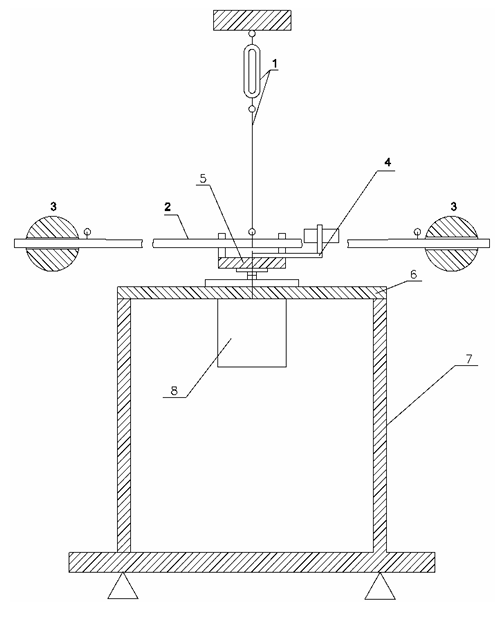
\includegraphics[scale=0.8]{stand} 
	}
	\legend{1 – система обезвешивания; 2 – штанга; 3 – груз; 4 – датчик угловой скорости с кронштейном для установки; 5 – элемент для передачи момента на выходной вал; 6 – плита установочная; 7 – основание; 8 – объект контроля}
	\caption{Функциональная схема инерционного стенда}
	\label{fig:stand} 
\end{figure}

Метод определения возмущающего момента, реализованный в работе Гончарука и соавт., %todo переписать соавторов
основан на использовании инерционного стенда, позволяющего воспроизводить динамические характеристики системы наведения антенн космического аппарата в наземных условиях. Конструктивно стенд представляет собой основание с закреплённой на нём плитой, на которой устанавливается механический привод антенны. К выходному валу привода присоединяется имитатор нагрузки, выполненный в виде штанги с грузами, масса и положение которых подбираются таким образом, чтобы эквивалентный момент инерции соответствовал параметрам реальной антенны. Для снижения влияния силы тяжести используется система обезвешивания, а инерционный имитатор позволяет воспроизводить упругие и динамические свойства навешиваемого оборудования.Регистрация параметров движения осуществляется с помощью датчика угловой скорости, установленного непосредственно на выходном валу привода. В процессе эксперимента фиксируется изменение угловой скорости при различных режимах работы — как при равномерном вращении, так и в переходных процессах разгона и торможения. Полученные зависимости $\omega(t)$ подвергаются дифференцированию для вычисления углового ускорения, после чего возмущающий момент определяется по выражению:
\begin{equation}
	\label{eq:eq_M_disturb}
	M=J_{\text{н}}\cdot \frac{d\omega}{dt}
\end{equation}

где \(J_{\text{н}}\) "--- момент инерции имитируемой нагрузки, \(\omega\) "--- угловая скорость.

Таким образом, метод сводиться к регистрации динамики вращения исполнительного механизма и последующему вычислению возмущающего момента через известные параметры имитируемой нагрузки.

Применение данного метода позволяет оценить возмущающее воздействие, создаваемое приводом в установившихся и переходных режимах, а также проанализировать их спектральные характеристики.

Несмотря на несомненные достоинства, описанный метод имеет ряд ограничений, которые не позволяют использовать его в рамках настоящего исследования. Прежде всего следует отметить, что стенд оперирует не реальной нагрузкой, а её имитатором, выполненным в виде штанги с грузами. Для каждой конкретной аппаратуры требуется изготавливать отдельный имитатор с заданным моментом инерции, и даже при тщательной калибровке всегда сохраняется погрешность в воспроизведении динамических характеристик реального узла. Кроме того, сам принцип измерений остаётся локальным: возмущающий момент определяется по данным датчика, установленного на валу привода, тогда как для \colorbox{yellow}{задач космической техники} критическим является именно реактивный момент, передаваемый на корпус КА. Такой подход не позволяет получить полное представление суммарном воздействии на конструкцию в реальных условиях работы. Наконец, существенным ограничением является невозможность воспроизведения ситуации, когда одновременно вращаются и нагрузка, и компенсирующий маховик. Регистрация реактивного момента после компенсации имеет принципиальное значение для оценки качества динамики в высокоточных оптико-электронных системах. В совокупности, эти факторы делают метод, реализованный на инерциальном стенде, недостаточным для решения поставленной в настоящей работе.

\section{Выводы по главе 1}
В первой главе рассмотрено современное состояние исследований в области динамических воздействий на оптико-электронные системы космических аппаратов и их влияние на качество формируемых изображений. Показано, что повышение разрешающей способности и внедрение механизмов поворота визирной оси без разворота аппарата сопровождается ростом требований к устойчивости изображения и одновременно приводит к усилению динамических возмущений, вызванных перемещением подвижных масс.

Анализ показал, что реактивный момент, возникающий в результате работы приводов, является одним из ключевых факторов, снижающих качество изображений. Его влияние проявляется через три компоненты: низкочастотную, гармоническую и случайную. Все они приводят к смещению скорости движения изображения на фокальной плоскости относительно оптимального значения, что вызывает смаз и дрожание изображения, а также снижает интегральные показатели качества, включая функцию передачи модуляции и Image Quality Factor.

Для снижения воздействия реактивного момента применяются различные методы компенсации, включая компенсирующие маховики, двухприводные механизмы, балансировочные устройства и алгоритмическую компенсацию на уровне законов управления. Эти решения позволяют уменьшить спектр возмущений в критических диапазонах частот, однако полностью устранить их влияние не удаётся. В системе неизбежно остаётся остаточный реактивный момент, который требует учёта и оценки.

Обзор существующих методов измерения крутящего момента показал, что они в основном ориентированы на регистрацию момента на валу двигателя. Такой подход отражает только локальное крутильное воздействие и не эквивалентен реактивному моменту, передаваемому на корпус космического аппарата. Рассмотренный метод экспериментальной отработки на инерционном стенде позволяет оценить возмущающие моменты привода, однако он основан на использовании имитатора нагрузки и не учитывает работу компенсирующих маховиков, а потому не позволяет регистрировать остаточный реактивный момент всей системы.

Таким образом, выполненный анализ подтвердил, что в доступной литературе практически отсутствуют исследования, посвящённые непосредственному измерению реактивного момента подвижных частей оптико-электронной аппаратуры космического назначения. Этот пробел обосновывает необходимость разработки специализированных методов регистрации и анализа остаточного реактивного момента, что и составляет предмет настоящего исследования.

\FloatBarrier

